% intro/motivation and outline of section
The goal of ultrasound reconstruction is to visualize the resulting data. Conventional ultrasound scans offer only a 2D view in the direction the ultrasound probe is pointing, but through a reconstructed volume, slices in any direction can be obtained. Furthermore, volume rendering techniques can give an overview of the area of interest in three dimensions, akin to looking into the body itself. This section explains two common visualization techniques for reconstructed ultrasound volumes. The first is multiplanar reformatting slices through the volume, and the second is volume rendering by ray casting.

% what are MPR slices?
\subsection{Multiplanar Reformatting Slices}

	Multiplanar reformatting (MPR) is a technique for generating sagittal, coronal, and oblique views from otherwise one-axial sections \cite{preim2007, fenster2002}. Parts of the human body can be difficult, if not impossible, to scan in any direction, such as down the length of the torso. Also, when scanning a brain covered in ultrasound-resistant bone skull, only a small surgically-made hole will provide a spot for the probe, not giving much freedom of movement. With MPR, one is able to generate slices in any arbitrary direction. Typically, three orthogonal directions are sufficient for clinical utility. Figure \ref{fig:mpr_slices} shows an example of MPR. Notice how all three dimensions (width, height and depth) can be seen.
	
	\begin{figure}[h]
	\centering
	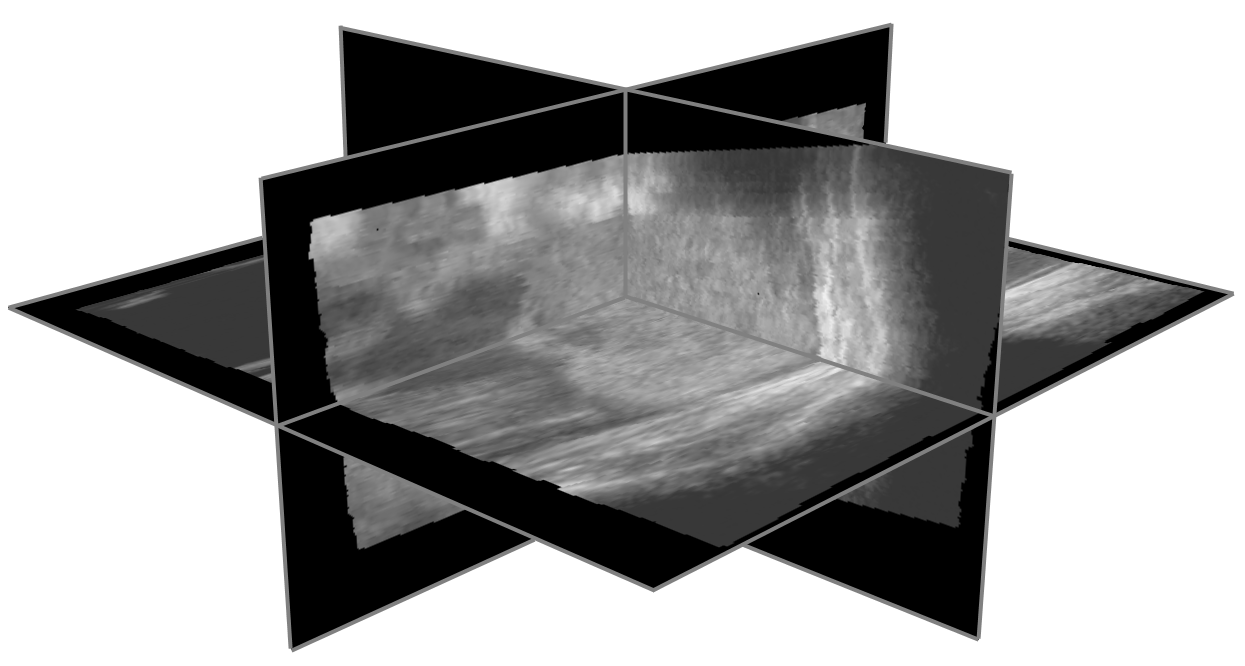
\includegraphics[height=0.3\textheight]{graphics/mpr_slices.png}
	\caption[Multiplanar reformatting of ultrasound]{Multiplanar reformatting of ultrasound (generated by our implementation)}
	\label{fig:mpr_slices}
	\end{figure}
	
	The MPR slices can be generated directly without constructing an actual volume, and this is demonstrated in the Stradx system \cite{prager1998}. But, the reconstructed volume is useful for other purposes such as volume rendering and storing offline for later use. In this thesis, we choose to obtain the MPR slices from a reconstructed volume.
	
	% Perhaps explain the orthogonal slices in implementation?
	%Orthogonal MPR-slices can be merged in the same coordinate system as seen in \ref{fig:orthogonal_slices}
	
	%\begin{figure}[h]
	%\centering
	%\includegraphics[height=\textwidth]{graphics/orthogonal_slices.png}
	%\caption{Orthogonal_MPR slices}
	%\label{fig:orthogonal_slices}
	%\end{figure}

% what is ray casting and how does it work?
\subsection{Volume Ray Casting}
	
	Ray casting is a technique where thousands of rays, one for each rendered pixel, are cast towards the scene \cite{preim2007, ludvigsen2010}. When the rays intersect the geometry they accumulate color, similar to how light rays work in nature, only in reverse. An example of a ray casted volume is given in Figure \ref{fig:ray_casting}. The technique is suitable for rendering volumes without a defined surface, but that are defined by a massive "cloud" of voxels. An alternative is to extract a surface by thresholding the voxel values and constructing facets on it by such algorithms as marching cubes \cite{lorensen1987}. However, with noisy data such as ultrasound scans, it is difficult to extract the exact surface \cite{sakas1995}. A better approach may be to render all voxels so that trained medical personnel can use their expert knowledge and experience to interpret the visualized data.
	
		
	\begin{figure}[h]
	\centering
	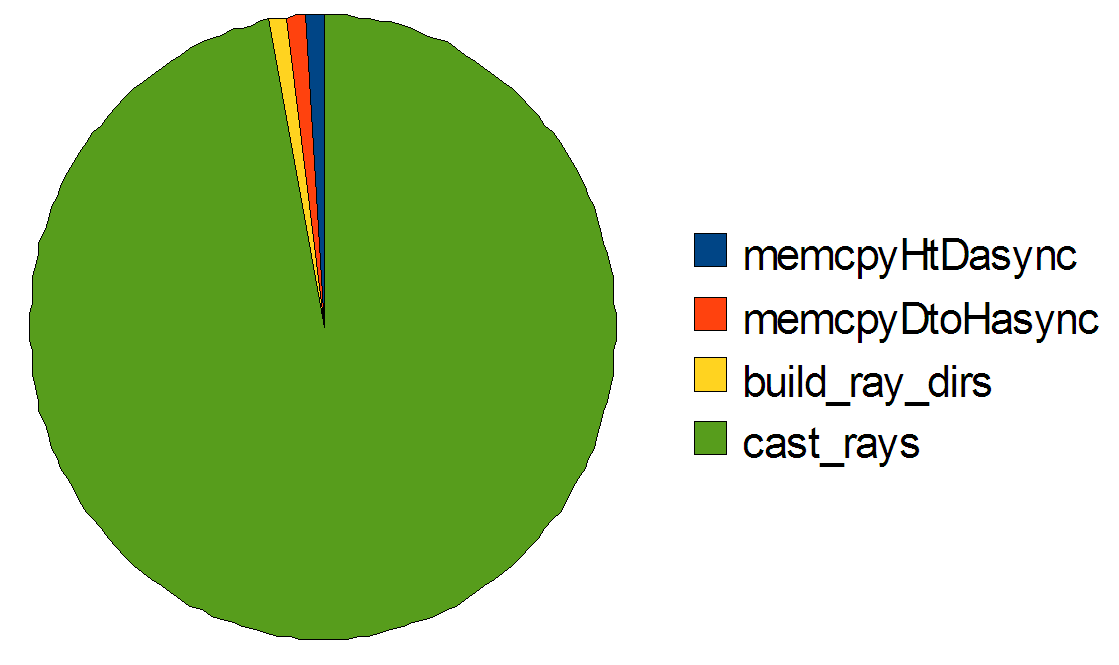
\includegraphics[height=0.35\textheight]{graphics/ray_casting.png}
	\caption[Ray casted render of fractal volume]{A ray casted render of a fractal volume (from our previous work \cite{ludvigsen2010})}
	\label{fig:ray_casting}
	\end{figure}
	
	The volume ray casting algorithm can be described as follows (based on \cite{preim2007}):
	
	\begin{itemize}
		\item for each ray:
		\begin{itemize}
			\item step along the ray direction in small incremental steps
			\item for each step:
			\begin{itemize}
				\item if inside a voxel, sample the volume and accumulate the value
			\end{itemize}
		\end{itemize}
	\end{itemize}
	
	Several methods for accumulating the voxel values exist, ranging from trivial addition, to complex estimation of how light is absorbed by mass in nature. Each ray has a defined origin (the camera position) and direction (determined by field-of-view and camera direction). The step size should ideally be such that each voxel is sampled only once and no voxel in the ray's path is missed, i.e.\ a step size larger than the distance between two neighbor voxels along an axis, and lower than the distance between two neighboring voxels along the diagonal.